\problemname{Pyramidbygge}

\begin{figure}[h!]
\centering
    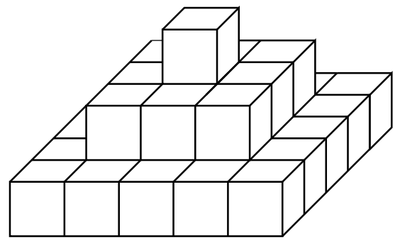
\includegraphics[width=0.6\textwidth]{pyramid.png}
  \caption{Ett exempel på en pyramid av höjd 3 med 35 block.}
\label{fig:pyramid}
\end{figure}

När man ska inleda ett större projekt, exempelvis bygga en pyramid, är det bäst att tänka efter en gång extra.
Du ska skriva ett program som beräknar hur hög pyramid man kan bygga om man har tillgång till ett visst antal stenblock.

Vi antar att pyramiden är kompakt, d.v.s. det finns inga hålrum inuti.
Vidare byggs den enligt principen i figur~\ref{fig:pyramid}.
Varje lager är alltså kvadratiskt med en sidlängd som är två block mindre än det underliggande lagrets.
Det översta lagret består alltid av ett ensamt block.

Det gör ingenting om det blir block över, men det får inte saknas ett enda block.

\section*{Indata}
Indata består av ett enda heltal $N$ ($1 \le N \le 100\,000\,000$): antal tillgängliga block.

\section*{Utdata}
Programmet ska skriva ut en rad med ett heltal: höjden för den största pyramid som kan byggas med som högst $N$ block.

\section*{Poängsättning}
Din lösning kommer att testas på en mängd testfallsgrupper.
För att få poäng för en grupp så måste du klara alla testfall i gruppen.


\noindent
\begin{tabular}{| l | l | p{12cm} |}
  \hline
  \textbf{Grupp} & \textbf{Poäng} & \textbf{Gränser} \\ \hline
  $1$    & $33$        & Det kommer inte bli några block över efter att pyramiden byggts. \\ \hline
  $2$    & $67$        & Inga ytterligare begränsningar. \\ \hline
\end{tabular}
